
%=========================================================================%

\subsection{Inverse Prediction}
Inverse prediction concerns predicting one set of measurements from another set when the direction of causation and possibly error operates in the opposite direction. An example is that of calibration in which it is desired to use a cheap and quick but error-prone measurement Y, to predict the true amount of a constituent x, which in itself can be measured accurately in laboratory conditions but at much greater effort or cost. After taking data on samples using both measurements (the training or learning data) it is desired to use the cheap measurement in future.


%=========================================================================%
\subsection{Quality Control}
c) A quality control process monitors the weight per carton of laundry detergent. 
Control limits for the mean are set at UCL = 20.12 ounces and LCL = 19.90 ounces. 
Samples of size 5 are used for the sampling and inspection process.

i) What are the process mean and process standard deviation for the manufacturing operation?

ii) If the process mean shifts to 20.25 ounces, what is the probability of a type II error? 	
   
%=========================================================================%


UVSA = c(84.63,84.38,84.08,84.41,83.82,83.55,83.92,83.69,84.06,84.03) 
NIRS = c(83.15,83.72,83.84,84.20,83.92,84.16,84.02,83.60,84.13,84.24)
mean(UVSA)
sd(UVSA)
mean(NIRS)
sd(NIRS)


t.test(UVSA)
t.test(UVSA, conf.level = 0.95)
t.test(UVSA, conf.level = 0.99)
t.test(NIRS)
t.test(NIRS, conf.level = 0.95)
t.test(NIRS, conf.level = 0.99)

CWdiff = UVSA–NIRS
t.test(UVSA, NIRS, paired= TRUE)


%=========================================================================%
\subsection{One Way ANOVA}

Six analysts each made seven determinations of the paracetamol content of the same batch of tablets.
The results are shown below
Analyst Paracetamol content
A 84.32 84.51 84.63 84.61 84.64 84.51 84.62
B 84.24 84.25 84.41 84.13 84.00 84.30 84.02
C 84.29 84.40 84.68 84.28 84.40 84.36 84.63
D 84.14 84.22 84.02 84.48 84.27 84.33 84.22
E 84.50 83.88 84.49 83.91 84.11 84.06 83.99
F 84.70 84.17 84.11 84.36 84.61 83.81 84.15
The following table has been produced as a result of analysis of these data:




X= c(19, 9.10000038146973, 9.19999980926514, 9.39999961853027, 9.39999961853027, 
9.5, 9.60000038146973, 9.60000038146973, 9.89999961853027, 9.89999961853027, 
10, 10.1000003814697, 10.3000001907349, 10.3999996185303, 10.6000003814697, 
10.6000003814697, 10.6000003814697, 10.6999998092651, 10.8000001907349, 
10.8000001907349, 10.8000001907349, 10.8000001907349, 10.8999996185303, 
10.8999996185303, 11, 11.1000003814697, 11.1000003814697, 11.1999998092651, 
11.3000001907349, 11.3999996185303, 11.3999996185303, 11.5, 11.5, 
11.6999998092651, 11.8000001907349, 12, 12.1000003814697, 12.1000003814697, 
12.3000001907349, 12.3999996185303, 12.5, 12.6999998092651, 13, 
13, 13.8000001907349, 14.3000001907349, 14.6999998092651, 14.8999996185303, 
18.3999996185303, 19.3999996185303, 22.1000003814697, 22.1000003814697
)


Y=c(1700, 114, 126, 138, 178, 208, 208, 261, 264, 282, 286, 301, 
402, 418, 434, 456, 326, 327, 339, 372,  463, 489, 496, 503, 504, 
515, 567, 593, 627, 761, 762, 766,  635, 679, 686, 715, 723, 744, 
780, 998, 1023, 1062,792, 805, 875, 930, 960,  1074, 1078, 1206, 
1500, 2922)

plot(X,Y)

plot(X,Y,col="red",pch=16,font.axis=2,font.lab=2)

FittedModel = lm(Y~X)

abline(coef(FittedModel))

influence(FittedModel)


> anova(FittedModel)
Analysis of Variance Table

Response: Y
          	Df  	Sum Sq 	Mean Sq 	F value    	Pr(>F)    
X         	 1 	9160239 	9160239 	 214.55 	< 2.2e-16 ***
Residuals 	50 	2134710   	42694                      
---
Signif. codes:  0 ‘***’ 0.001 ‘**’ 0.01 ‘*’ 0.05 ‘.’ 0.1 ‘ ’ 1 


%=================%
\subsection{Question}
Six analysts each made seven determinations of the paracetamol content of the same batch of tablets.
The results are shown below
Analyst Paracetamol content
A 84.32 84.51 84.63 84.61 84.64 84.51 84.62
B 84.24 84.25 84.41 84.13 84.00 84.30 84.02
C 84.29 84.40 84.68 84.28 84.40 84.36 84.63
D 84.14 84.22 84.02 84.48 84.27 84.33 84.22
E 84.50 83.88 84.49 83.91 84.11 84.06 83.99
F 84.70 84.17 84.11 84.36 84.61 83.81 84.15
The following table has been produced as a result of analysis of these data:




X= c(19, 9.10000038146973, 9.19999980926514, 9.39999961853027, 9.39999961853027, 
9.5, 9.60000038146973, 9.60000038146973, 9.89999961853027, 9.89999961853027, 
10, 10.1000003814697, 10.3000001907349, 10.3999996185303, 10.6000003814697, 
10.6000003814697, 10.6000003814697, 10.6999998092651, 10.8000001907349, 
10.8000001907349, 10.8000001907349, 10.8000001907349, 10.8999996185303, 
10.8999996185303, 11, 11.1000003814697, 11.1000003814697, 11.1999998092651, 
11.3000001907349, 11.3999996185303, 11.3999996185303, 11.5, 11.5, 
11.6999998092651, 11.8000001907349, 12, 12.1000003814697, 12.1000003814697, 
12.3000001907349, 12.3999996185303, 12.5, 12.6999998092651, 13, 
13, 13.8000001907349, 14.3000001907349, 14.6999998092651, 14.8999996185303, 
18.3999996185303, 19.3999996185303, 22.1000003814697, 22.1000003814697
)


Y=c(1700, 114, 126, 138, 178, 208, 208, 261, 264, 282, 286, 301, 
402, 418, 434, 456, 326, 327, 339, 372,  463, 489, 496, 503, 504, 
515, 567, 593, 627, 761, 762, 766,  635, 679, 686, 715, 723, 744, 
780, 998, 1023, 1062,792, 805, 875, 930, 960,  1074, 1078, 1206, 
1500, 2922)

plot(X,Y)

plot(X,Y,col="red",pch=16,font.axis=2,font.lab=2)

FittedModel = lm(Y~X)

abline(coef(FittedModel))

influence(FittedModel)


> anova(FittedModel)
Analysis of Variance Table

Response: Y
          	Df  	Sum Sq 	Mean Sq 	F value    	Pr(>F)    
X         	 1 	9160239 	9160239 	 214.55 	< 2.2e-16 ***
Residuals 	50 	2134710   	42694                      
---
Signif. codes:  0 ‘***’ 0.001 ‘**’ 0.01 ‘*’ 0.05 ‘.’ 0.1 ‘ ’ 1 

%=========================================================================%

\subsection{One Wayt ANOVA}
Five standard solutions were prepared, each containing $18.00\%$ (by weight) of chloride. Four titration methods were used to analyse each standard solution. The order of the experiments was randomized. The results of each procedures are tabulated below:
\begin{center}
    \begin{tabular}{|c|c|c|c|c|}
      \hline
      % after \\: \hline or \cline{col1-col2} \cline{col3-col4} ...

      Solution &  Method A & Method B & Method C & Method D \\\hline
1	&	18.03	&	18.13	&	18.09	&	18.14	\\
2	&	18.05	&	18.13	&	18.15	&	18.11	\\
3	&	18.02	&	17.94	&	18.12	&	18.12	\\
4	&	18.12	&	17.97	&	18.10	&	18.04	\\
5	&	18.22	&	18.00	&	18.08	&	18.02	\\

      \hline
    \end{tabular}
    \end{center}
The following output is the result of performing a two-way ANOVA procedure in \texttt{R}.
\begin{framed}
\begin{verbatim}
            Df  Sum Sq  Mean Sq F value Pr(>F)
Method       3 0.01498 0.004993   0.934  0.454
Solution     4 0.01043 0.002607   0.488  0.745
Residuals   12 0.06417 0.005347
\end{verbatim}
\end{framed}

%Solution = structure(c(1L, 2L, 3L, 4L, 5L, 1L, 2L, 3L, 4L, 5L, 1L, 2L, 3L,
%4L, 5L, 1L, 2L, 3L, 4L, 5L), .Label = c("1", "2", "3", "4", "5"), class = "factor")
%Method=structure(c(1L, 1L, 1L, 1L, 1L, 2L, 2L, 2L, 2L, 2L, 3L, 3L, 3L,
%3L, 3L, 4L, 4L, 4L, 4L, 4L), .Label = c("A", "B", "C", "D"), class = "factor")



\begin{itemize}
\item[i.] (2 marks) Determine whether there is a significant difference between the concentration of chloride in different solutions.
\item[ii.] (2 marks) Determine whether there is a  significant difference obtained by the different titration methods.
\end{itemize}

\item[(b)] A review of the data revealed that there were two replicate measurements for each combination of method and solution. The revised data is tabulated below.

    \begin{tabular}{|c|c|c|c|c|}
      \hline
      % after \\: \hline or \cline{col1-col2} \cline{col3-col4} ...

      Solution &  Method A & Method B & Method C & Method D \\\hline
1&	18.03, 18.06	&	18.13, 18.15	&	18.09, 18.11	&	18.14, 18.16	\\
2&	18.05, 18.07	&	18.13, 18.14	&	18.15, 18.18	&	18.11, 18.13	\\
3&	18.02, 18.04	&	17.94, 17.97	&	18.12, 18.15	&	18.12, 18.12	\\
4&	18.12, 18.14	&	17.97, 17.98	&	18.10, 18.13	&	18.04, 18.07	\\
5&	18.22, 18.19	&	18.00, 18.02	&	18.08, 18.11	&	18.02, 18.09	\\
      \hline
    \end{tabular}

\begin{framed}
\begin{verbatim}
                Df  Sum Sq  Mean Sq F value   Pr(>F)
Solution         4 0.02083 0.005209   13.44 1.78e-05 ***
Method           3 0.03349 0.011163   28.81 1.85e-07 ***
Solution:Method 12 0.10563 0.008802   22.71 4.86e-09 ***
Residuals       20 0.00775 0.000387
---
Signif. codes:  0 ‘***’ 0.001 ‘**’ 0.01 ‘*’ 0.05 ‘.’ 0.1 ‘ ’ 1
\end{verbatim}
\end{framed}

\begin{itemize}
\item[i.] (4 Marks) Explain how the revised data set is
\item[ii.] (2 marks) Determine whether there is a significant difference between the concentration of chloride in different solutions, based on the revised data.
\item[iii.] (2 marks) Determine whether there is a  significant difference obtained by the different titration methods, based on the revised data.

\end{itemize}




\begin{center}
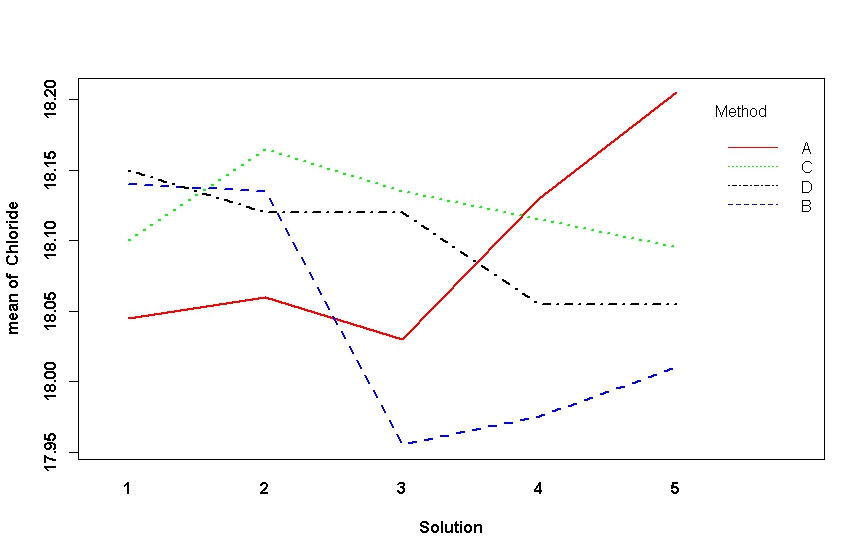
\includegraphics[scale=0.45]{ExamQ6interaction}
\end{center}
\newpage

\begin{verbatim}




DAT2 = c(90, 100, 90, 120, 110, 100, 100, 160, 70, 120, 110, 150, 100, 
130, 80, 140)

DAT1 = DAT2/10

A=c("L", "H", "L", "H", "L", "H", "L", "H", "L", "H", "L", "H", "L", "H", "L", "H")
B=c("L", "L", "H", "H", "L", "L", "H", "H", "L", "L", "H", "H", "L", "L", "H", "H")
C=c("L", "L", "L", "L", "H", "H", "H", "H", "L", "L", "L", "L", "H", "H", "H", "H")



A=factor(A,c("L","H"))
B=factor(B,c("L","H"))
C=factor(C,c("L","H"))

Model2=aov(DAT1~A*B*C)
summary(Model2)

> summary(Model2)
            Df Sum Sq Mean Sq F value  Pr(>F)   
A            1   4556    4556  18.692 0.00253 **
B            1   1056    1056   4.333 0.07093 . 
C            1    306     306   1.256 0.29485   
A:B          1    756     756   3.103 0.11620   
A:C          1      6       6   0.026 0.87675   
B:C          1    156     156   0.641 0.44646   
A:B:C        1    506     506   2.077 0.18751   
Residuals    8   1950     244                   
---
Signif. codes:  0 ‘***’ 0.001 ‘**’ 0.01 ‘*’ 0.05 ‘.’ 0.1 ‘ ’ 1 
> DAT1=DAT2/10
> Model1=aov(DAT1~A*B*C)
> summary(Model1)
            Df Sum Sq Mean Sq F value  Pr(>F)   
A            1  45.56   45.56  18.692 0.00253 **
B            1  10.56   10.56   4.333 0.07093 . 
C            1   3.06    3.06   1.256 0.29485   
A:B          1   7.56    7.56   3.103 0.11620   
A:C          1   0.06    0.06   0.026 0.87675   
B:C          1   1.56    1.56   0.641 0.44646   
A:B:C        1   5.06    5.06   2.077 0.18751   
Residuals    8  19.50    2.44                   
---
Signif. codes:  0 ‘***’ 0.001 ‘**’ 0.01 ‘*’ 0.05 ‘.’ 0.1 ‘ ’ 1 
\end{verbatim}



